\documentclass[tikz,border=0pt]{standalone}
\usepackage{pgfplots}
\usepackage{xcolor}

% original colors
\definecolor{color1}{RGB}{166,118,29}
\definecolor{color2}{RGB}{217,95,2}
\definecolor{color3}{RGB}{231,41,138}
\definecolor{color4}{RGB}{117,112,179}
\definecolor{color5}{RGB}{27,158,119}
\definecolor{color6}{RGB}{102,166,30}
\definecolor{color7}{RGB}{230,171,2}

\begin{document}
\begin{tikzpicture}
\node[inner sep=0pt]  at (0,0)
    {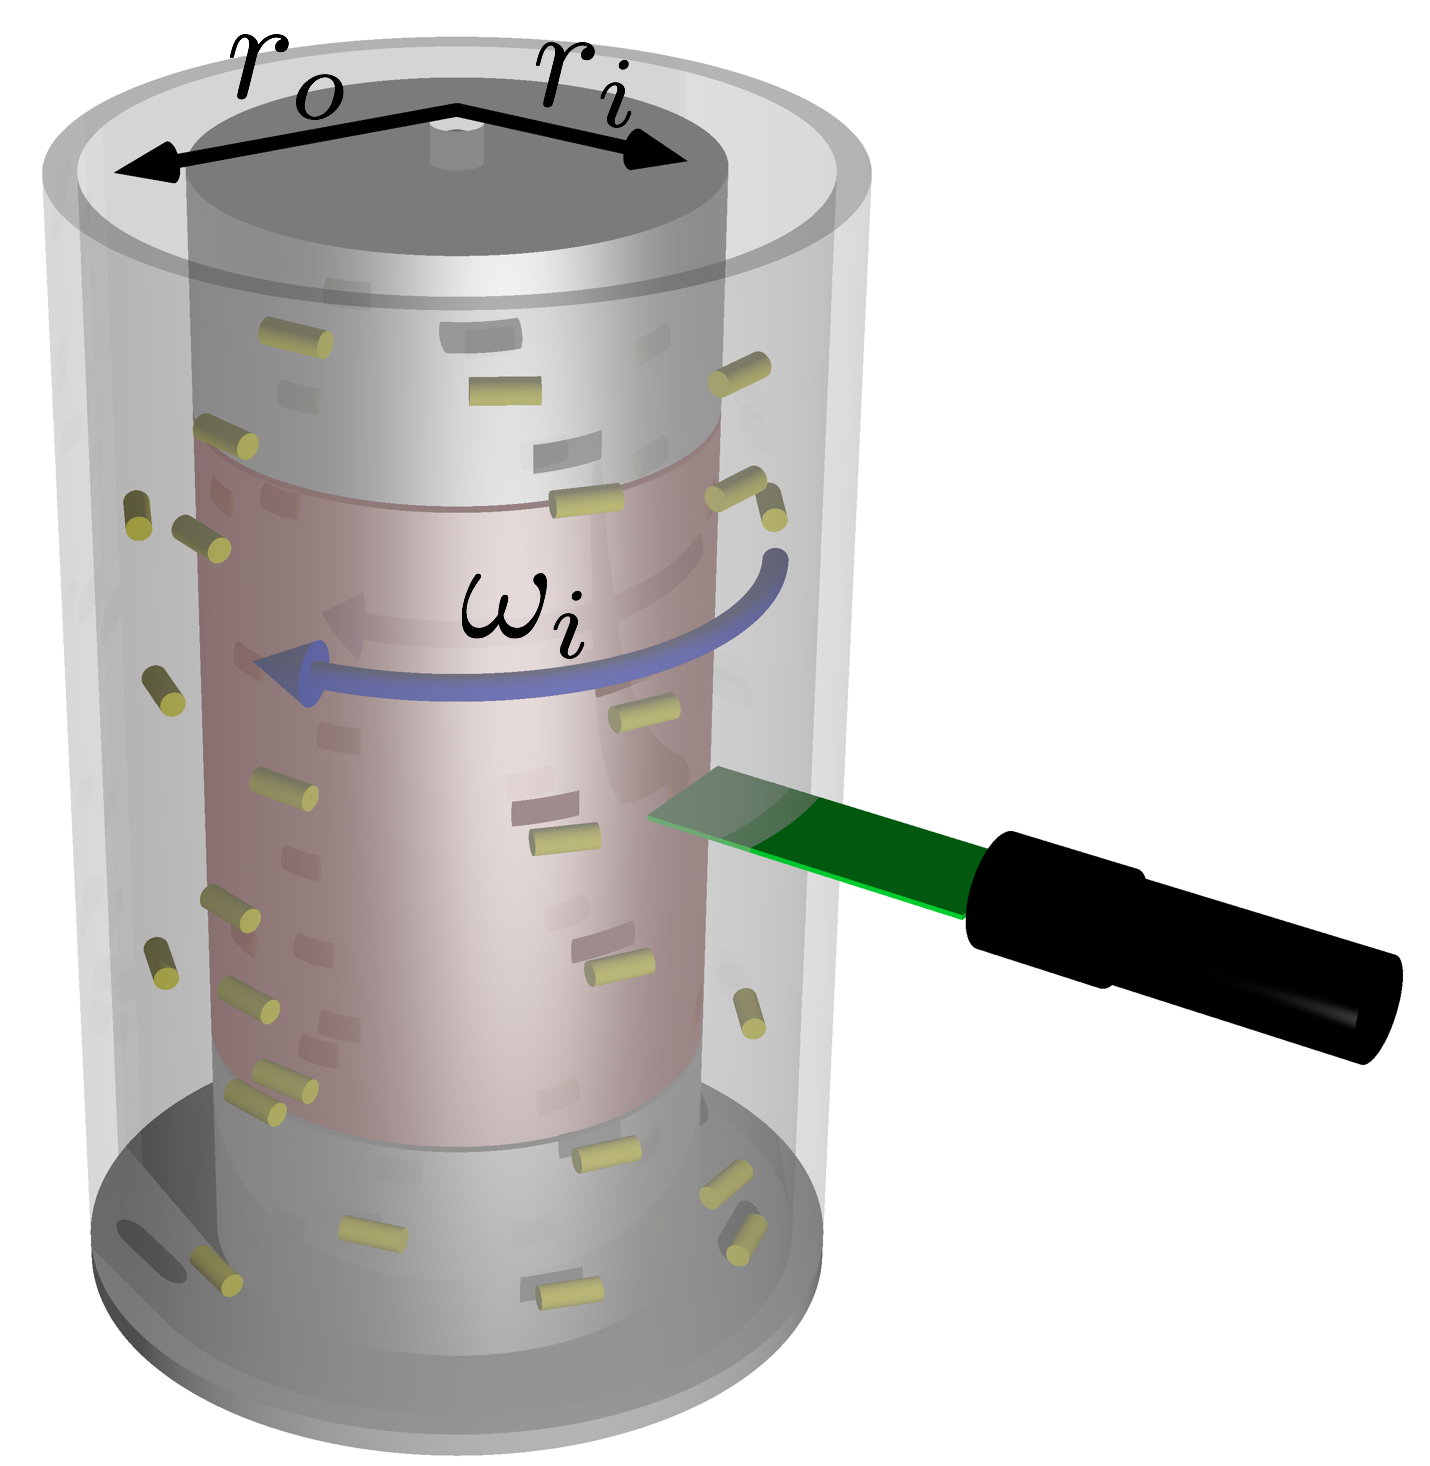
\includegraphics[height=7cm]{figure1asetup.png}};
\node at (-3.5, 3.25) {(a)};
\end{tikzpicture}
\end{document}
